\tikzset{>=latex} % for LaTeX arrow head
\contourlength{1.6pt}
\colorlet{Bcol}{violet!90}
\colorlet{BFcol}{red!60!black}
\colorlet{veccol}{green!45!black}
\colorlet{Icol}{blue!70!black}
\tikzstyle{BField}=[->,very thick,Bcol]
\tikzstyle{current}=[->,Icol] %thick,
\tikzstyle{force}=[->,very thick,BFcol]
\tikzstyle{velocity}=[->,very thick,vcol]
\tikzstyle{charge+}=[very thin,draw=black,top color=red!50,bottom color=red!90!black,shading angle=20,circle,inner sep=0.5]
\tikzstyle{charge-}=[very thin,draw=black,top color=blue!50,bottom color=blue!80,shading angle=20,circle,inner sep=0.5]
\tikzstyle{vector}=[->,thick,veccol]
\tikzset{
  BFieldLine/.style={thick,Bcol,decoration={markings,mark=at position #1 with {\arrow{latex}}},
                     postaction={decorate}},
  BFieldLine/.default=0.5,
  pics/Bin/.style={
    code={
      \def\R{0.12}
      \draw[pic actions,Bcol,line width=0.6] % ,thick
        (0,0) circle (\R) (-135:.7*\R) -- (45:.7*\R) (-45:.7*\R) -- (135:.7*\R);
  }},
}

% B FIELD horizontal, zero velocity




% B FIELD horizontal, top view


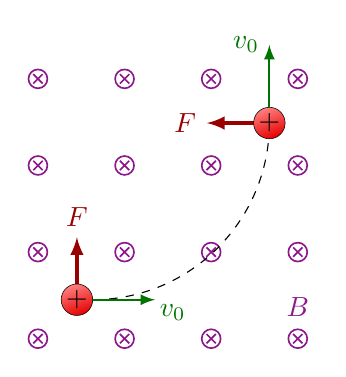
\begin{tikzpicture}
  \def\xmax{3.3}
  \def\ymax{3.3}
  \def\R{0.2}
  \def\P{0.68*\xmax}
  \def\v{0.24*\xmax}
  \def\F{0.18*\xmax}
  \def\NBy{4}
  \def\NBx{4}
  \coordinate (Q) at (0.15*\xmax,0.15*\ymax);
  
  % MAGNETIC FIELD
  \foreach \i [evaluate={\y=(\i-1)*\ymax/(\NBy-1);}] in {1,...,\NBy}{
    \foreach \i [evaluate={\x=(\i-1)*\xmax/(\NBx-1);}] in {1,...,\NBx}{
      \pic[rotate=-90] at (\x,\y) {Bin};
    }
  }
  \node[Bcol] at (\xmax,0.12*\ymax) {$\vb{B}$};
  
  % CHARGE
  \draw[dashed] (Q)++(\R,0) arc (-90:0:\P) coordinate (F);
  \draw[vector] (Q)++(\R,0) --++ (\v,0) node[below right=-2] {$\vb{v}_0$};
  \draw[vector] (F)++(0,\R) --++ (0,\v) node[left=0] {$\vb{v}_0$};
  \draw[force]  (Q)++(0,\R) --++ (0,\F) node[above=0] {$\vb{F}$};
  \draw[force]  (F)++(-\R,0) --++ (-\F,0) node[left=0] {$\vb{F}$};
  \draw[charge+] (Q) circle (\R) node {$+$};
  \draw[charge+] (F) circle (\R) node {$+$};
  
\end{tikzpicture}
